\chapter{Convolutional Neural Networks}\label{ch:cnn}
Convolutional Neural Network (CNN) is a class of Artificial Neural Networks\footnote{A computational model inspired by
animal brain.}, which allows for efficient training on high dimensional data.
This is especially useful in the field of computer vision as image data is fundamentally high dimensional.

Architecture of CNNs contains many layers.
Because of that, these models belong the class of machine learning methods called
\textit{deep learning}\footnote{Set of machine learning models with \textit{credit assignment path (CAP)} higher than 2.
The CAP is the chain of transformations from input to output.}
In the following section~\ref{sec:layer-types} I will deal with layer types used in CNNs.

\begin{figure}[H]
    \centering
    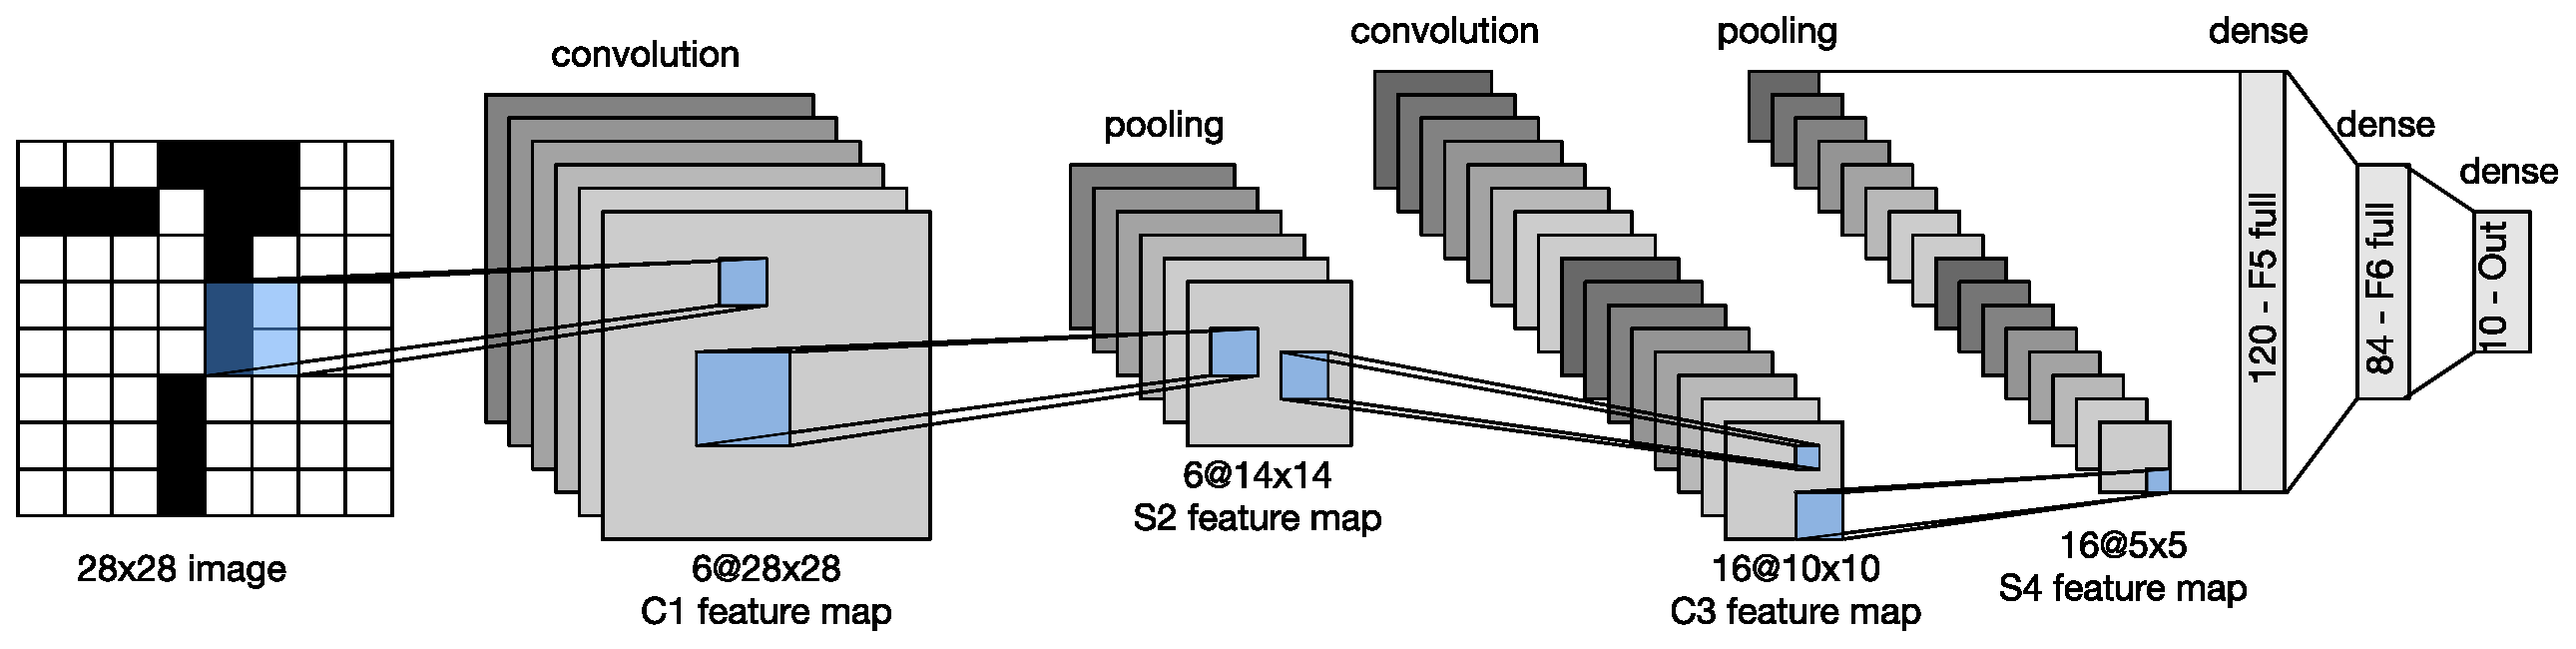
\includegraphics[width=\columnwidth]{images/cnn/lenet.eps}
    \caption{Example of CNN model (LeNet 5)~\cite{LeNet5}}
    \label{fig:cnn}
\end{figure}

\section{Layer Types}\label{sec:layer-types}
The image~\ref{fig:cnn} is an illustration of one of the oldest CNN models, called \textit{LenNet 5}, which was used for
handwritten character recognition.

As we can see there are three layer types: \textit{dense}~\ref{sec:dense},
\textit{convolutional}~\ref{sec:convolutional} and \textit{pooling}~\ref{sec:pooling}.

\subsection{Dense}\label{sec:dense}
Dense layer is the simplest type of layer present in CNN models.
Its output is determined simply by multiplication of \textit{inputs} (x) with \textit{weight matrix}
(denoted V in~\ref{eq:dense}, also called kernel) and addition of \textit{bias} (u).

\begin{equation}
    \label{eq:dense}
    h[i, j] = u[i,j] + \sum_{a,b} V[i,j,a,b] \cdot x[i+a,j+b]
\end{equation}

Now let's imagine, that we have greyscale image which is 256 pixel wide and high as an input.
If we flatten the image to a vector, we get input with $256\cdot256 = 65536$ dimensions.
Even if we do aggressive reduction to 1000 hidden dimensions, we end up with ~65 million parameters.
This makes dense layer impractical when dealing with imagery and that's when convolution~\ref{sec:convolutional} comes
into play.

\subsection{Convolutional}\label{sec:convolutional}
As I hinted in the previous section, the main advantage of CNNs~\cite{ConvLayer} is the low amount of parameters needed.
In the convolutional layer this feat was achieved by application of two principles:
\textit{invariance}~\ref{subsec:invariance} and \textit{locality}~\ref{subsec:locality}.

\subsubsection{Invariance Principle}\label{subsec:invariance}
The core of invariance principle is reuse of the weights.
This is achieved by application of the weights on one part of the image, shifting the weights by a predetermined set
of pixels (called stride) and then applying the weights again.
Let us examine the equation~\ref{eq:denseinv} too see how the original equation~\ref{eq:dense} changes.

\begin{equation}
    \label{eq:denseinv}
    h[i, j] = u + \sum_{a,b} V[a,b] \cdot x[i+a,j+b]
\end{equation}

As is to be expected, bias \textit{u} and the weight matrix \textit{V} are no longer dependent upon the image
coordinates \textit{(i, j)}.
As an example we can think of an airplane detection algorithm whose objective is to find whether there is an airplane
in arbitrary location of the scene.
We would do that by sliding one set of weights describing the airplane over the image.
The algorithm would classify the scene with high impulse response as containing the airplane.
This intuitively makes a lot of sense.

This type of invariance is called \textit{translational invariance}.

\subsubsection{Locality Principle}\label{subsec:locality}
Another principle used in CNNs is so called \textit{locality principle}.
This principle suggests, that we do not need to look far away from \textit{(i,j)} to gain valuable information about
what is going on in that particular location.
This is achieved, mathematically speaking, by limiting \textit{a} and \textit{b} to a range $\Delta$.

\begin{equation}
    \label{eq:denseinvloc}
    h[i, j] = u + \sum_{a=-\Delta}^{\Delta} \sum_{b=-\Delta}^{\Delta} V[a,b] \cdot x[i+a,j+b]
\end{equation}

Equation~\ref{eq:denseinvloc} is the final form describing the convolution layer.

\subsection{Pooling}\label{sec:pooling}
The main objective of pooling is to decrease the spatial dimension of the inner representation of the data.
During classification (the most common application of CNNs) we are not interested in the location of the classified
object within the image.
The only information that interests us is whether the object is present in the scene or not.
With this information in mind pooling~\cite{PoolingLayer} was invented.

Pooling layer is similar to convolutional layer in a sense that both are "looking" only at a part of the input at once.
This point of view (window) is then shifted as I described in the section~\ref{subsec:invariance}.
The difference is that there is no kernel present in the operation.
The only thing pooling does is that it selects/computes the most representative value from the window.
There are two common pooling types: \textit{max pooling} and \textit{average pooling}.
The first type selects the maximum value and the second one computes average.

Stacking pooling layer on top of convolutional layer is a powerful combination as pooling effectively filters out
impulse responses corresponding to noise.

\section{Padding}\label{subsec:padding}
To avoid loss of information at the edges of the image we usually use a method called \textit{padding}.
This technique increases the image dimension by pixel addition around the original image.
There are few padding variants which are differentiated by the value of the new pixels.
The most common ones are \textit{zero padding} and \textit{reflective padding}.
The first mentioned type, as the name implies, sets the new pixels to zero.
The second one is more sophisticated and consists in mirroring of the neighboring pixels.

\section{Use Cases}\label{sec:use-cases}
As I mentioned in the beginning of the chapter, CNNs are mainly used in the field of
\textit{computer vision}\footnote{Scientific field dealing with extraction of high level understanding from imagery
using computers.}.
This theses is dealing with a subset of computer vision called \textit{face recognition}\ref{ch:face-rec} in which CNNs
achieve state of the art results.
For this reason, this chapter is present in the text.